\documentclass{beamer}
\usepackage[utf8]{inputenc}
\title{QTBrowser}
\subtitle{Superimposing arbitrary plots \\and accessing DQM GUI files}
\author{\texorpdfstring{Filip Ilic\newline\url{filip.ilic@cern.ch}}{Filip ilic}}
\date{\today}

\begin{document}
\maketitle

\begin{frame}
  \frametitle{Motivation}
	
	\begin{itemize}
\item<1-> Limitations of DQM GUI
    \begin{itemize}
        \item GUI only allows superimposing / overlaying the same plots across different runs.
        \item Superimposing arbitrary plots would be useful.
    \end{itemize}
    
\item Ease of Use
    \begin{itemize}
        \item Downloading files through the DQM GUI is more complicated than it has to be.
    \end{itemize}
\item Make macros reusable
	\begin{itemize}
	\item There's a lot of ROOT macros written and then discarded (and probably rewritten multiple times by different people).
	\item QTBrowser offers a way to make your macros available to others through plugins.
	\end{itemize}	
\end{itemize}
\end{frame}

\begin{frame}
\frametitle{QTBrowser - File Browser}
  \begin{columns}[T]
    \begin{column}{.5\textwidth}
     \begin{block}{}
     \begin{itemize}
     \item Can open .root files, and search within them for plots.
     \item Different modes which provide functionality when plots are selected.
     \end{itemize}
    	\end{block}	
    \end{column}
    \begin{column}{.5\textwidth}
    \begin{block}{}
% Your image included here
    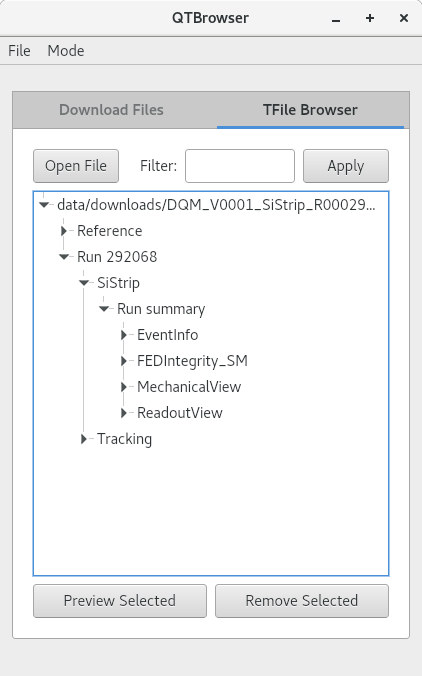
\includegraphics[width=.7\textwidth]{figures/browser_view.png}
    \end{block}
    \end{column}
  \end{columns}
\end{frame}



\begin{frame}
\frametitle{QTBrowser - Modes}
  \begin{columns}[T]
    \begin{column}{.5\textwidth}
     \begin{block}{}
     \begin{itemize}
          \item Current modes:
     	\begin{itemize}
     		\item Superimpose
     		\item Concatenate
     		\item Fit
		\end{itemize}   
     \item Clicking on one of the modes extends the area.
     \item Items that are now clicked in the file browser will be sent to the plugin, which can perform its task.
  	 
     \end{itemize}

    	\end{block}	
    \end{column}
    \begin{column}{.5\textwidth}
    \begin{block}{}
% Your image included here
    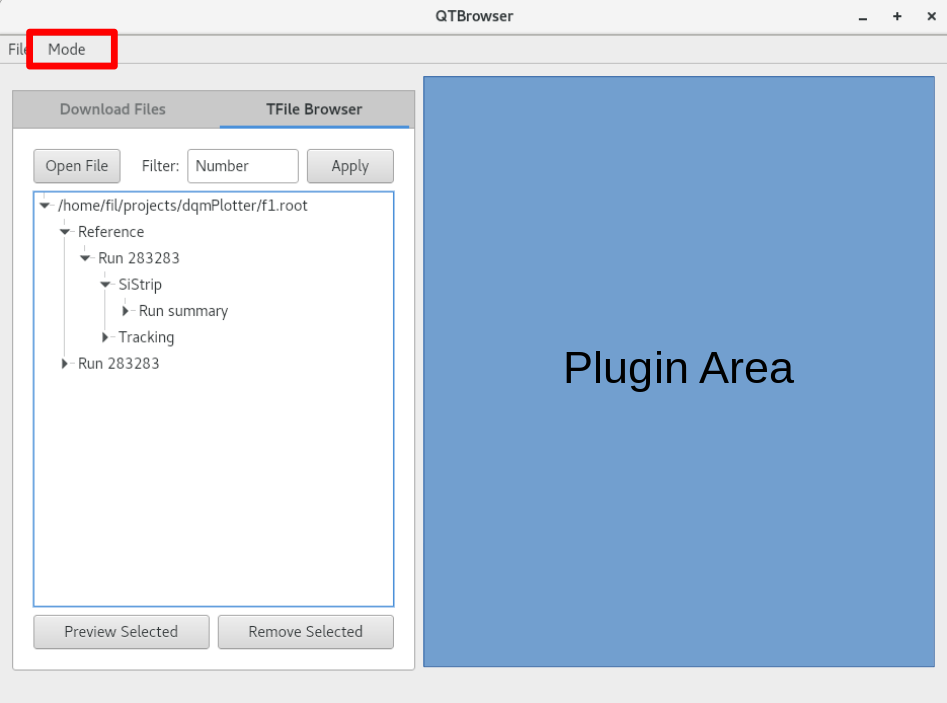
\includegraphics[width=\textwidth]{figures/plugin_area.png}
    \end{block}
    \end{column}
  \end{columns}
\end{frame}



\begin{frame}
\frametitle{Modes - Superimpose}
  \begin{columns}[T]
    \begin{column}{.5\textwidth}
     \begin{block}{}
     \begin{itemize}
     \item Double clicking items in the file browser adds them to the plugin.
     \item The selected plots are drawn in the top right, the superimposition in the bottom panel.
     \item There is no limit on how many plots can be superimposed.
     \end{itemize}
   	\end{block}	
    \end{column}
    \begin{column}{.5\textwidth}
    \begin{block}{}
% Your image included here
    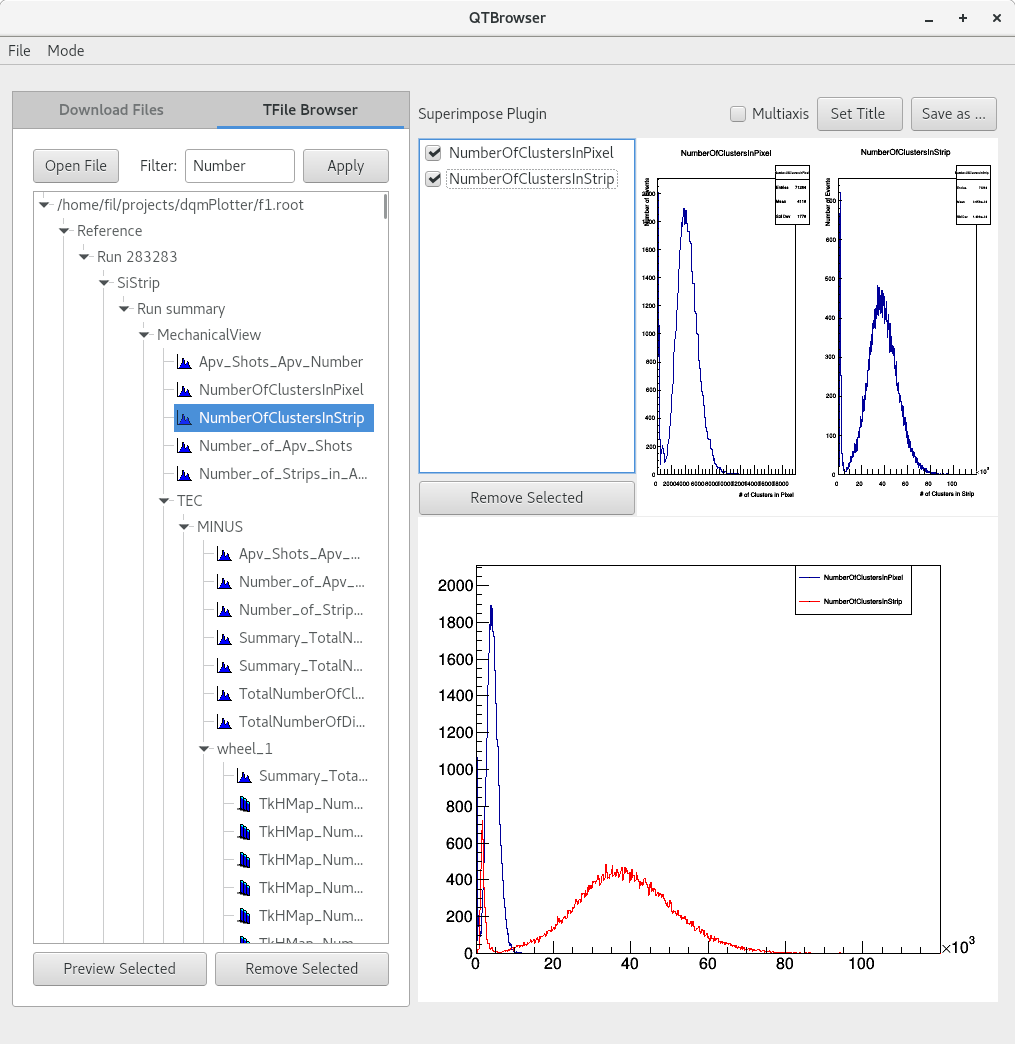
\includegraphics[width=\textwidth]{figures/superimpose.png}
    \end{block}
    \end{column}
  \end{columns}
\end{frame}

\begin{frame}
\frametitle{Modes - Superimpose}
  \begin{columns}[T]
    \begin{column}{.5\textwidth}
     \begin{block}{}
     \begin{itemize}
     \item Double clicking items in the file browser adds them to the plugin.
     \item The selected plots are drawn in the top right, the superimposition in the bottom panel.
     \item There is no limit on how many plots can be superimposed.
     \end{itemize}
   	\end{block}	
    \end{column}
    \begin{column}{.5\textwidth}
    \begin{block}{}
% Your image included here
    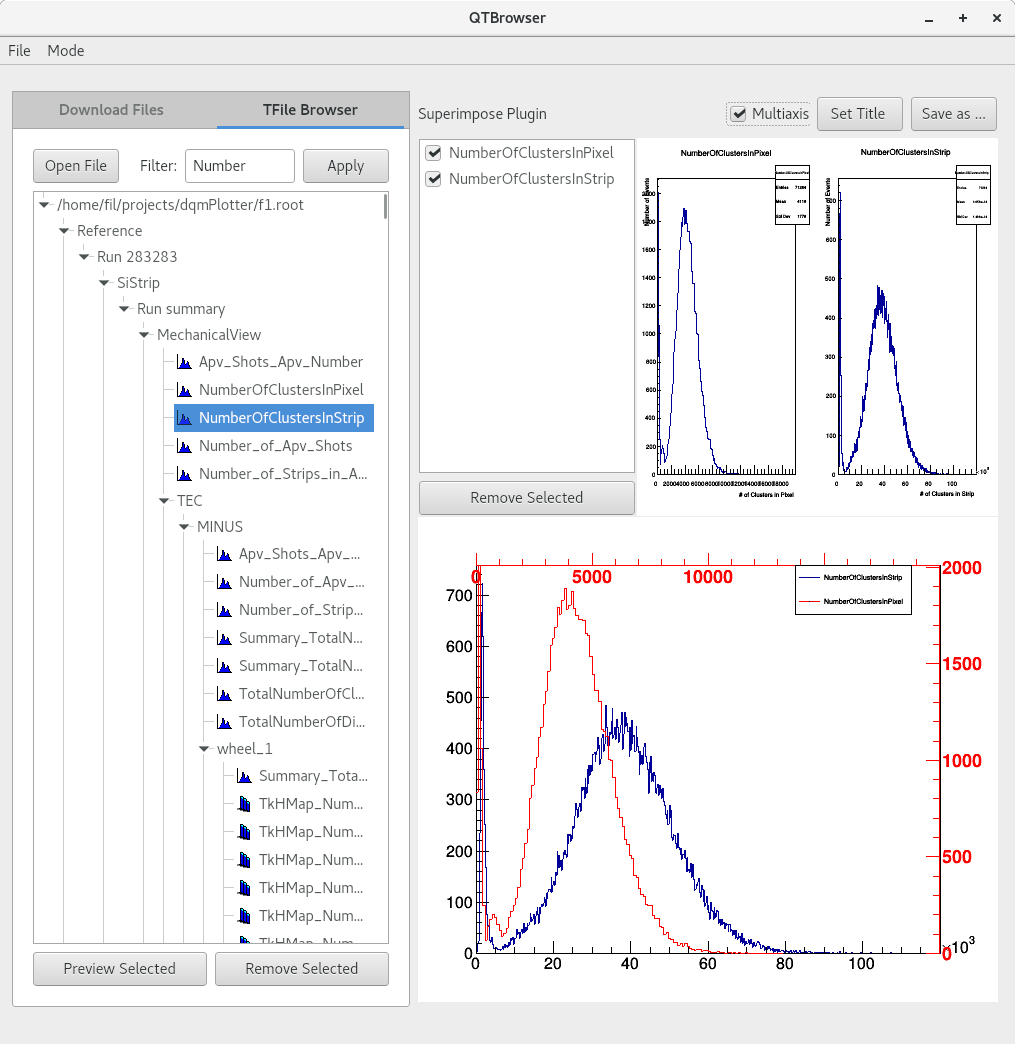
\includegraphics[width=\textwidth]{figures/superimpose_multiaxis.png}
    \end{block}
    \end{column}
  \end{columns}
\end{frame}



\begin{frame}
\frametitle{Modes - Fit}
	\begin{center}
    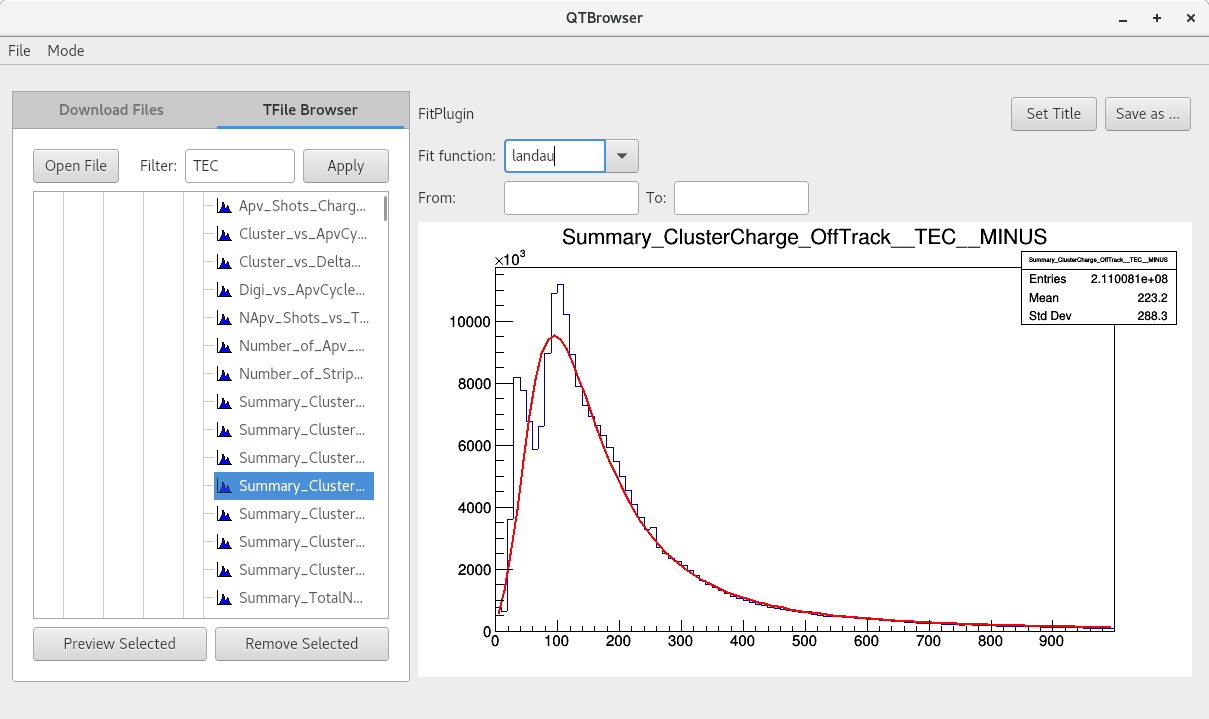
\includegraphics[width=0.7\textwidth]{figures/fit.png}
    \end{center}
Fitting distributions to plots.
\end{frame}



\begin{frame}
\frametitle{Modes - Concatenate}
	\begin{center}
    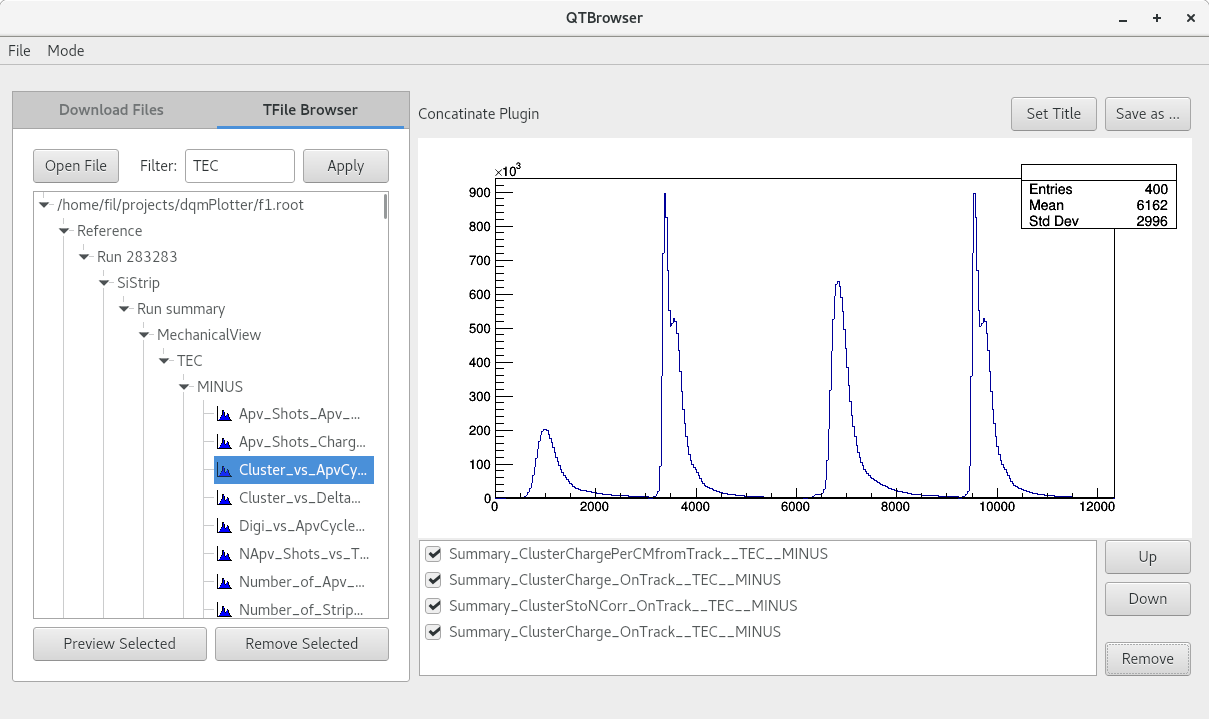
\includegraphics[width=0.7\textwidth]{figures/concat.png}
    \end{center}
Concatenating plots
\end{frame}


\begin{frame}
\frametitle{QTBrowser - Downloader}
  \begin{columns}[T]
    \begin{column}{.5\textwidth}
     \begin{block}{}
     \begin{itemize}
     \item Browse Online, Offline, Relval files from DQM GUI.
     \item Download files with a single click.
     \item Valid grid certificate needed.
     \item Keeping index of files up to date; still work in progress (as of 30.11.2017).
     \end{itemize}
   	\end{block}	
    \end{column}
    \begin{column}{.5\textwidth}
    \begin{block}{}
% Your image included here
    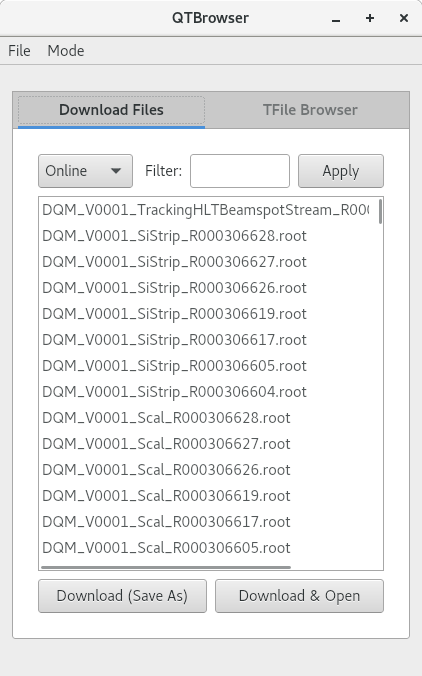
\includegraphics[width=0.7\textwidth]{figures/downloader.png}
    \end{block}
    \end{column}
  \end{columns}
\end{frame}

\begin{frame}
\frametitle{How to run it}
Remotely on vocms61:
\begin{itemize}
\item \texttt{ssh cctrack@vocms061.cern.ch -Y}
\item \texttt{cd /data/users/filic/}
\item \texttt{cd CMSSW\_9\_4\_0 \&\& cmsenv \&\& cd ..}
\item \texttt{./updateOnlineIndex \&\& ./startQTBrowser}
\end{itemize}
Locally:
\begin{itemize}
\item Currently you will need to compile it
\item Linux and macOs: instructions in the README.
\item Windows: work in progress. (as of 1.12.2017)
\end{itemize}

\end{frame}

\begin{frame}
\frametitle{Sidenote - creating new pulgins}
 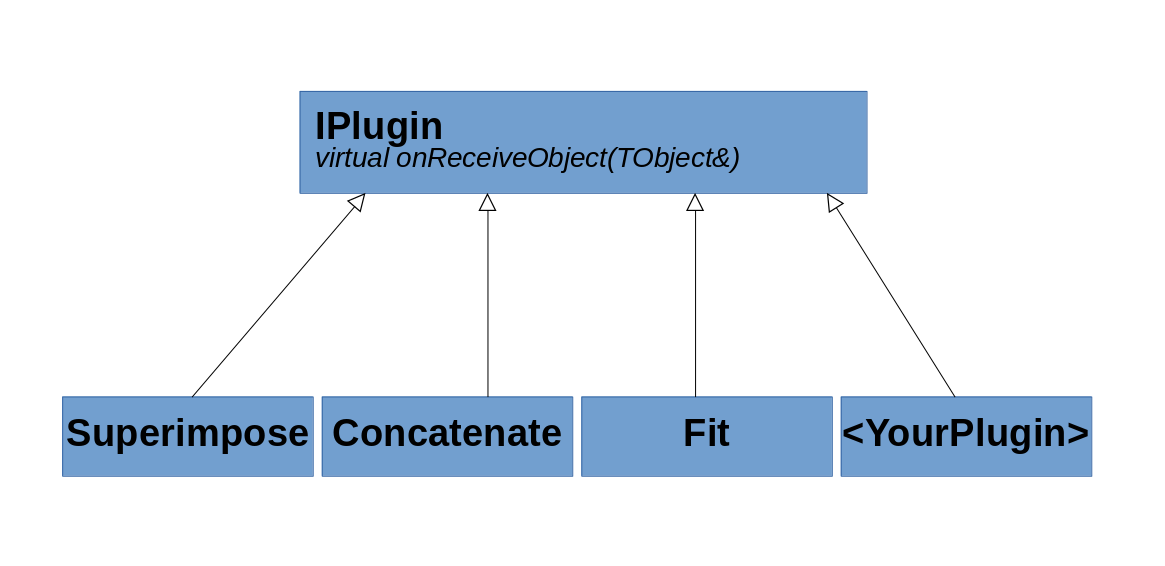
\includegraphics[width=0.7\textwidth]{figures/iplugin_uml.png}
 \begin{itemize}
 \item It is straight forward to add your own plugin.
 \item All that needs to be done is deriving from IPlugin and implementing the virtual functions
 for your plugin to receive TObjects from the file browser.
 \end{itemize}
\end{frame}

\begin{frame}
\begin{itemize}
\item Repository: https://github.com/imKuehlschrank/QTBrowser
\item Suggestions/Feedback: filip.ilic@cern.ch
\end{itemize}
\end{frame}

\end{document}